The purpose of this chapter is to provide quantitative upper and lower-bound estimates on the expected electron flux due to LEP, as a function of location and time of year. We expand on the raytracing and interpolation method described in chapter \ref{chapter:power}, by incorporating a resonant-particle scattering code. We compute global electron fluxes in a similar manner as in chapter \ref{chapter:power}, using an array of precomputed stencils, which we scale and shift according to GLD360 data. Finally, we can examine the relative timescales on which LEP could deplete a populated magnetic field line, in the absence of any other loss processes.





\paragraph{Where should you put the magnetosphere statistics? that big correlation plot of kp, ae, Dst, etc etc}

\section{LEP stencils}
\label{section:lep_stencils}
\section{Coordinate deformation}
The stencils in section \ref{section:lep_stencils} are computed using a dipole magnetic field, and the simplified GCPM model, both to reduce computational complexity and to better generalize to multiple longitudes. However, we can approximate the effect of a more-complex magnetic field model via a coordinate transformation, in which we rotate input coordinates to an equivalent dipole-model coordinate, and perform an inverse operation on the stencil output. On the stencil output, this approximation is justified by noting that trapped electrons are bound to their respective field lines, regardless of model used. Justification on the input side (deforming the input coordinates of a lightning flash) is less-concrete, but still a reasonable assumption. First, experimentation with the raytracer reveals that, given a longitudinally-symmetric plasma density model, rays generally follow the longitude deviation of the magnetic field model. Second, while the IGRF and Dipole models differ greatly in its footprint on the ground (as in figure \ref{fig:Lshell_example}), within the plasmasphere the two models have reasonable agreement (as in figure \ref{fig:fieldline_example}).

The \emph{Corrected Geomagnetic Coordinate} (CGM) \citep{Hakura1965} system is especially well-suited for this task. CGM coordinates are defined by fieldline tracing between the IGRF and Dipole models. To transform from geographic to CGM coordinates, we first trace a fieldline using IGRF from the surface, up to its intersection with the geomagnetic equatorial plane. We then follow the dipole model back down to the surface, to get an equivalent dipole-model coordinate. The inverse transformation is accomplished by following the dipole field line back up to the equator, and the IGRF model down to its footprint \citep{Laundal2016}.

Field line tracing is a computationally-intensive task for a coordinate transformation tool. Historically, researchers relied on precomputed lookup tables and interpolation. The Altitude-Adjusted CGM (AACGM) model \citep{Baker1989, Shepherd2014} uses a spherical-harmonic fit to rapidly transform between CGM and MAG coordinates.

CGM coordinate systems are undefined at some regions near the geomagnetic equator, due to the fact that some IGRF fieldlines may never intersect with it. In these cases, approximate models are often used. \cite{Baker1989} simply omitted geomagnetic latitudes within $\sim 24^\circ$ of the equator from their study; subsequent researchers have performed spline fits and interpolation to further reduce the undefined region.

We use the algorithm and implementation from \cite{Shepherd2014}, available at \emph{http://superdarn.thayer.dartmouth.edu/aacgm.html}. Figure \ref{fig:CGM_globe_comparison} compares MAG and AACGM contours on a geographic map.

% Our study already excludes these latitudes on the basis that below $\sim 20^\circ$ geomagnetic latitude, field lines do not exit the ionosphere at their apex.




\begin{figure}[ht]
\begin{center}
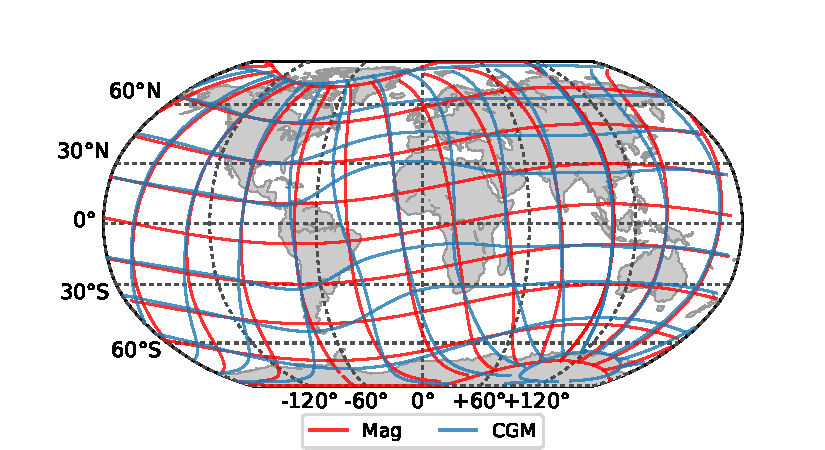
\includegraphics{figures/CGM_globe_comparison.pdf}
\caption[Comparison of Magnetic Dipole (MAG) and Corrected Geomagnetic (CGM) coordinates]{A comparison between Magnetic Dipole (MAG) and Corrected Geomagnetic (CGM) coordinates. Corrected Geomagnetic coordinates are obtained by following a magnetic field line, as defined by IGRF, from an input point to its intersection with the magnetic dipole equator. The CGM latitude and longitude are then obtained by following the dipole field line to its footprint on the Earth's surface. Contours are spaced every $20^\circ$ in geomagnetic latitude, and $30^\circ$ in geomagnetic longitude.}
\label{fig:CGM_globe_comparison}
\end{center}
\end{figure}

\section{Global and Seasonal Energy Fluxes}

\section{Lifetime Estimates}